\documentclass[12pt]{article} % 
\usepackage{fontspec} %To handle the font named Sans Forgetica
\usepackage{lipsum} %For generating dummy text.
\usepackage{graphicx} %To handle images in the document.

% Created by Jamie Cropley
% http://jamie.zone



\setmainfont{[SansForgetica-Regular.otf]} %To load the font named Sans Forgetica




\begin{document}


\begin{flushleft}
%Any text I have goes here for one paragraph, in place of lipsum.
\section*{Title for first paragraph:}
\lipsum[1]
\end{flushleft}


\begin{flushleft}
%For a new paragraph write it here in place of lipsum.
\section*{Title for second paragraph:}
\lipsum[1]
\end{flushleft}


%For a new page:
\newpage


\begin{flushleft}
%For lists:
\section*{Title for lists:}
\begin{itemize}
  \item One entry in the list
  \item Another entry in the list
  \begin{itemize}
  \item Sub item example 1
  \item Sub item example 2
  \begin{itemize}
  \item A sub sub item 1
  \item A sub sub item 2
  \end{itemize}
  \end{itemize}
\end{itemize}
\end{flushleft}


%For a new page:
\newpage


% Putting in tabular data: https://www.overleaf.com/learn/latex/Tables


\begin{flushleft}
\section*{Planet Earth Image Title:}
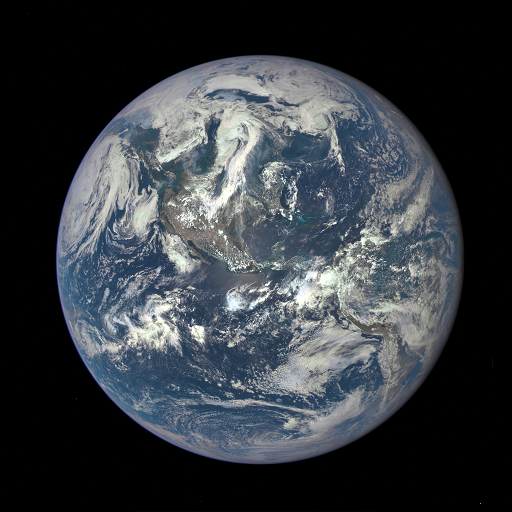
\includegraphics{earth.png} %I can replace this and put any image
\end{flushleft}


\end{document}